% Options for packages loaded elsewhere
\PassOptionsToPackage{unicode}{hyperref}
\PassOptionsToPackage{hyphens}{url}
\PassOptionsToPackage{dvipsnames,svgnames,x11names}{xcolor}
%
\documentclass[
  letterpaper,
  DIV=11,
  numbers=noendperiod]{scrartcl}

\usepackage{amsmath,amssymb}
\usepackage{iftex}
\ifPDFTeX
  \usepackage[T1]{fontenc}
  \usepackage[utf8]{inputenc}
  \usepackage{textcomp} % provide euro and other symbols
\else % if luatex or xetex
  \usepackage{unicode-math}
  \defaultfontfeatures{Scale=MatchLowercase}
  \defaultfontfeatures[\rmfamily]{Ligatures=TeX,Scale=1}
\fi
\usepackage{lmodern}
\ifPDFTeX\else  
    % xetex/luatex font selection
\fi
% Use upquote if available, for straight quotes in verbatim environments
\IfFileExists{upquote.sty}{\usepackage{upquote}}{}
\IfFileExists{microtype.sty}{% use microtype if available
  \usepackage[]{microtype}
  \UseMicrotypeSet[protrusion]{basicmath} % disable protrusion for tt fonts
}{}
\makeatletter
\@ifundefined{KOMAClassName}{% if non-KOMA class
  \IfFileExists{parskip.sty}{%
    \usepackage{parskip}
  }{% else
    \setlength{\parindent}{0pt}
    \setlength{\parskip}{6pt plus 2pt minus 1pt}}
}{% if KOMA class
  \KOMAoptions{parskip=half}}
\makeatother
\usepackage{xcolor}
\setlength{\emergencystretch}{3em} % prevent overfull lines
\setcounter{secnumdepth}{-\maxdimen} % remove section numbering
% Make \paragraph and \subparagraph free-standing
\ifx\paragraph\undefined\else
  \let\oldparagraph\paragraph
  \renewcommand{\paragraph}[1]{\oldparagraph{#1}\mbox{}}
\fi
\ifx\subparagraph\undefined\else
  \let\oldsubparagraph\subparagraph
  \renewcommand{\subparagraph}[1]{\oldsubparagraph{#1}\mbox{}}
\fi

\usepackage{color}
\usepackage{fancyvrb}
\newcommand{\VerbBar}{|}
\newcommand{\VERB}{\Verb[commandchars=\\\{\}]}
\DefineVerbatimEnvironment{Highlighting}{Verbatim}{commandchars=\\\{\}}
% Add ',fontsize=\small' for more characters per line
\usepackage{framed}
\definecolor{shadecolor}{RGB}{241,243,245}
\newenvironment{Shaded}{\begin{snugshade}}{\end{snugshade}}
\newcommand{\AlertTok}[1]{\textcolor[rgb]{0.68,0.00,0.00}{#1}}
\newcommand{\AnnotationTok}[1]{\textcolor[rgb]{0.37,0.37,0.37}{#1}}
\newcommand{\AttributeTok}[1]{\textcolor[rgb]{0.40,0.45,0.13}{#1}}
\newcommand{\BaseNTok}[1]{\textcolor[rgb]{0.68,0.00,0.00}{#1}}
\newcommand{\BuiltInTok}[1]{\textcolor[rgb]{0.00,0.23,0.31}{#1}}
\newcommand{\CharTok}[1]{\textcolor[rgb]{0.13,0.47,0.30}{#1}}
\newcommand{\CommentTok}[1]{\textcolor[rgb]{0.37,0.37,0.37}{#1}}
\newcommand{\CommentVarTok}[1]{\textcolor[rgb]{0.37,0.37,0.37}{\textit{#1}}}
\newcommand{\ConstantTok}[1]{\textcolor[rgb]{0.56,0.35,0.01}{#1}}
\newcommand{\ControlFlowTok}[1]{\textcolor[rgb]{0.00,0.23,0.31}{#1}}
\newcommand{\DataTypeTok}[1]{\textcolor[rgb]{0.68,0.00,0.00}{#1}}
\newcommand{\DecValTok}[1]{\textcolor[rgb]{0.68,0.00,0.00}{#1}}
\newcommand{\DocumentationTok}[1]{\textcolor[rgb]{0.37,0.37,0.37}{\textit{#1}}}
\newcommand{\ErrorTok}[1]{\textcolor[rgb]{0.68,0.00,0.00}{#1}}
\newcommand{\ExtensionTok}[1]{\textcolor[rgb]{0.00,0.23,0.31}{#1}}
\newcommand{\FloatTok}[1]{\textcolor[rgb]{0.68,0.00,0.00}{#1}}
\newcommand{\FunctionTok}[1]{\textcolor[rgb]{0.28,0.35,0.67}{#1}}
\newcommand{\ImportTok}[1]{\textcolor[rgb]{0.00,0.46,0.62}{#1}}
\newcommand{\InformationTok}[1]{\textcolor[rgb]{0.37,0.37,0.37}{#1}}
\newcommand{\KeywordTok}[1]{\textcolor[rgb]{0.00,0.23,0.31}{#1}}
\newcommand{\NormalTok}[1]{\textcolor[rgb]{0.00,0.23,0.31}{#1}}
\newcommand{\OperatorTok}[1]{\textcolor[rgb]{0.37,0.37,0.37}{#1}}
\newcommand{\OtherTok}[1]{\textcolor[rgb]{0.00,0.23,0.31}{#1}}
\newcommand{\PreprocessorTok}[1]{\textcolor[rgb]{0.68,0.00,0.00}{#1}}
\newcommand{\RegionMarkerTok}[1]{\textcolor[rgb]{0.00,0.23,0.31}{#1}}
\newcommand{\SpecialCharTok}[1]{\textcolor[rgb]{0.37,0.37,0.37}{#1}}
\newcommand{\SpecialStringTok}[1]{\textcolor[rgb]{0.13,0.47,0.30}{#1}}
\newcommand{\StringTok}[1]{\textcolor[rgb]{0.13,0.47,0.30}{#1}}
\newcommand{\VariableTok}[1]{\textcolor[rgb]{0.07,0.07,0.07}{#1}}
\newcommand{\VerbatimStringTok}[1]{\textcolor[rgb]{0.13,0.47,0.30}{#1}}
\newcommand{\WarningTok}[1]{\textcolor[rgb]{0.37,0.37,0.37}{\textit{#1}}}

\providecommand{\tightlist}{%
  \setlength{\itemsep}{0pt}\setlength{\parskip}{0pt}}\usepackage{longtable,booktabs,array}
\usepackage{calc} % for calculating minipage widths
% Correct order of tables after \paragraph or \subparagraph
\usepackage{etoolbox}
\makeatletter
\patchcmd\longtable{\par}{\if@noskipsec\mbox{}\fi\par}{}{}
\makeatother
% Allow footnotes in longtable head/foot
\IfFileExists{footnotehyper.sty}{\usepackage{footnotehyper}}{\usepackage{footnote}}
\makesavenoteenv{longtable}
\usepackage{graphicx}
\makeatletter
\def\maxwidth{\ifdim\Gin@nat@width>\linewidth\linewidth\else\Gin@nat@width\fi}
\def\maxheight{\ifdim\Gin@nat@height>\textheight\textheight\else\Gin@nat@height\fi}
\makeatother
% Scale images if necessary, so that they will not overflow the page
% margins by default, and it is still possible to overwrite the defaults
% using explicit options in \includegraphics[width, height, ...]{}
\setkeys{Gin}{width=\maxwidth,height=\maxheight,keepaspectratio}
% Set default figure placement to htbp
\makeatletter
\def\fps@figure{htbp}
\makeatother

\KOMAoption{captions}{tableheading}
\makeatletter
\makeatother
\makeatletter
\makeatother
\makeatletter
\@ifpackageloaded{caption}{}{\usepackage{caption}}
\AtBeginDocument{%
\ifdefined\contentsname
  \renewcommand*\contentsname{Table of contents}
\else
  \newcommand\contentsname{Table of contents}
\fi
\ifdefined\listfigurename
  \renewcommand*\listfigurename{List of Figures}
\else
  \newcommand\listfigurename{List of Figures}
\fi
\ifdefined\listtablename
  \renewcommand*\listtablename{List of Tables}
\else
  \newcommand\listtablename{List of Tables}
\fi
\ifdefined\figurename
  \renewcommand*\figurename{Figure}
\else
  \newcommand\figurename{Figure}
\fi
\ifdefined\tablename
  \renewcommand*\tablename{Table}
\else
  \newcommand\tablename{Table}
\fi
}
\@ifpackageloaded{float}{}{\usepackage{float}}
\floatstyle{ruled}
\@ifundefined{c@chapter}{\newfloat{codelisting}{h}{lop}}{\newfloat{codelisting}{h}{lop}[chapter]}
\floatname{codelisting}{Listing}
\newcommand*\listoflistings{\listof{codelisting}{List of Listings}}
\makeatother
\makeatletter
\@ifpackageloaded{caption}{}{\usepackage{caption}}
\@ifpackageloaded{subcaption}{}{\usepackage{subcaption}}
\makeatother
\makeatletter
\@ifpackageloaded{tcolorbox}{}{\usepackage[skins,breakable]{tcolorbox}}
\makeatother
\makeatletter
\@ifundefined{shadecolor}{\definecolor{shadecolor}{rgb}{.97, .97, .97}}
\makeatother
\makeatletter
\makeatother
\makeatletter
\makeatother
\ifLuaTeX
  \usepackage{selnolig}  % disable illegal ligatures
\fi
\IfFileExists{bookmark.sty}{\usepackage{bookmark}}{\usepackage{hyperref}}
\IfFileExists{xurl.sty}{\usepackage{xurl}}{} % add URL line breaks if available
\urlstyle{same} % disable monospaced font for URLs
\hypersetup{
  pdftitle={Matt Viana},
  colorlinks=true,
  linkcolor={blue},
  filecolor={Maroon},
  citecolor={Blue},
  urlcolor={Blue},
  pdfcreator={LaTeX via pandoc}}

\title{Matt Viana}
\author{}
\date{}

\begin{document}
\maketitle
\ifdefined\Shaded\renewenvironment{Shaded}{\begin{tcolorbox}[sharp corners, borderline west={3pt}{0pt}{shadecolor}, boxrule=0pt, frame hidden, breakable, enhanced, interior hidden]}{\end{tcolorbox}}\fi

\hypertarget{ds-220}{%
\subsubsection{DS 220}\label{ds-220}}

\hypertarget{section}{%
\subsubsection{12/7/2023}\label{section}}

\hypertarget{correlation-of-wages-in-different-education-levels-and-consumer-price-index-from-2000-to-2022}{%
\section{Correlation of wages in different education levels and Consumer
Price Index from 2000 to
2022}\label{correlation-of-wages-in-different-education-levels-and-consumer-price-index-from-2000-to-2022}}

It has been in the public eye that the cost of living has dramatically
increased in the last 20 years. For the purpose of enriching my data
analytical skills and knowledge of relevant issues for a student about
to enter the workforce, I decided to track two metrics of cost of
living. The analysis of trends in wages distributed by differences in
levels of education, in addition to the inflation rates since the year
2000 provides an important base case representative of the value of
money for working Americans. This analysis holds significant importance
due to its direct impact on standards of living, income distribution,
and overall economic health. The motivation behind this study stems from
the need to comprehend the evolving relationship between education,
wages, and inflation, which serves as a pivotal aspect in shaping
socioeconomic policies and guiding investments.

The focus of this analytical project is on two datasets. US Inflation
Dataset (1947 - 2023) where we will be surveying Consumer Price Index
variations, and Hourly Wages by Education in the USA (1973-2022) from
2000 - 2022. By correlating a significant and relevant span year over
year, it enables the creation of data models that display economic
trends. Using these models we aim to answer the following questions: How
much have wages increased in the measured timeframe? Have wages changed
consistently across the different levels of education?\\
How much has the CPI risen in the measured timeframe?\\
Has there been a consistent relationship between the CPI and wage growth
over the past two decades? What is the difference in purchasing power in
2000 to 2022 based on education levels? Which levels of education have
shown the strongest correlation between wage changes and CPI variations
since 2000? What are relevant trends displayed?

The correlation between education and wages has long been established,
yet the intricate nuances within this relationship, especially in the
context of fluctuating economic conditions represented by inflation,
remain a personal curiosity of mine. This exploration delves into the
changes in wage differentials across various education levels over the
past two decades, considering the overarching influence of inflationary
pressures on these earning differentials.

\hypertarget{recognizing-the-criteria}{%
\subsection{Recognizing the Criteria}\label{recognizing-the-criteria}}

Key concepts to be explored include the influence of education levels on
wage disparities, tracking individuals under these categories: Less than
a High School diploma, High School, College Degree, Bachelors Degree,
and Advanced Degree.

CPI is calculated based on a predetermined basket of goods and services
commonly purchased by urban consumers. This basket represents various
categories like housing, food, transportation, education, healthcare,
and entertainment. For the analyzed data set the information was
measured by the Federal Reserve Economic Data (FRED), Federal Reserve
Bank of St.~Louis. For this paper, the base CPI used to track
percentages is 2000-01-01, with a calculated CPI of 169.3. This means a
CPI of 200 represents approximately an 18.13\% increase from the base.

Leveraging the capabilities of Python's Pandas library as a statistical
tool has provided a robust framework for data manipulation, analysis,
and visualization. This comprehensive approach explores the interactions
between Consumer Price Index variations and wage trends across different
educational backgrounds. By delineating these criteria, we've
established a foundational understanding of the questions at hand.

Surveying the data An obvious starting point when pursuing this analysis
was determining the most basic metrics provided by the data. Looking at
the wage data, mapping the change in income over time for each category
shows the increase over the years and the difference between categories.

\begin{Shaded}
\begin{Highlighting}[]
\ImportTok{import}\NormalTok{ pandas }\ImportTok{as}\NormalTok{ pd}
\ImportTok{import}\NormalTok{ matplotlib.pyplot }\ImportTok{as}\NormalTok{ plt}


\NormalTok{CPI }\OperatorTok{=}\NormalTok{ pd.read\_csv(}\StringTok{"US\_inflation\_rates.csv"}\NormalTok{)}
\NormalTok{wages }\OperatorTok{=}\NormalTok{ pd.read\_csv(}\StringTok{"wages\_by\_education.csv"}\NormalTok{)}

\CommentTok{\#Clean Data, remove duplicates and empty rows}
\NormalTok{CPI }\OperatorTok{=}\NormalTok{ CPI.dropna()}
\NormalTok{wages }\OperatorTok{=}\NormalTok{ wages[::}\OperatorTok{{-}}\DecValTok{1}\NormalTok{]}
\NormalTok{wages }\OperatorTok{=}\NormalTok{ wages.dropna()}
\NormalTok{wages }\OperatorTok{=}\NormalTok{ wages.drop\_duplicates()}

\CommentTok{\# Limited the data from the year 2000 to 2022}
\NormalTok{CPI }\OperatorTok{=}\NormalTok{ CPI[CPI[}\StringTok{\textquotesingle{}value\textquotesingle{}}\NormalTok{] }\OperatorTok{\textgreater{}} \FloatTok{169.3}\NormalTok{]}
\NormalTok{CPI }\OperatorTok{=}\NormalTok{ CPI[CPI[}\StringTok{\textquotesingle{}value\textquotesingle{}}\NormalTok{] }\OperatorTok{\textless{}} \FloatTok{298.99}\NormalTok{]}
\NormalTok{CPI[}\StringTok{\textquotesingle{}date\textquotesingle{}}\NormalTok{] }\OperatorTok{=}\NormalTok{ pd.to\_datetime(CPI[}\StringTok{\textquotesingle{}date\textquotesingle{}}\NormalTok{])}

\NormalTok{wages }\OperatorTok{=}\NormalTok{ wages[wages[}\StringTok{\textquotesingle{}year\textquotesingle{}}\NormalTok{] }\OperatorTok{\textgreater{}} \DecValTok{1999}\NormalTok{]}
\NormalTok{wages }\OperatorTok{=}\NormalTok{ wages.iloc[:, :}\DecValTok{6}\NormalTok{]}


\NormalTok{wage\_years }\OperatorTok{=}\NormalTok{ wages[}\StringTok{\textquotesingle{}year\textquotesingle{}}\NormalTok{]}
\NormalTok{wages\_noYear }\OperatorTok{=}\NormalTok{ wages.drop(columns}\OperatorTok{=}\StringTok{\textquotesingle{}year\textquotesingle{}}\NormalTok{) }
\end{Highlighting}
\end{Shaded}

\begin{Shaded}
\begin{Highlighting}[]
\CommentTok{\# Plotting line graph 1}
\NormalTok{plt.figure(figsize}\OperatorTok{=}\NormalTok{(}\DecValTok{8}\NormalTok{, }\DecValTok{6}\NormalTok{))}
\ControlFlowTok{for}\NormalTok{ column }\KeywordTok{in}\NormalTok{ wages.columns:}
\NormalTok{    plt.plot(wage\_years, wages[column], label}\OperatorTok{=}\NormalTok{column)}

\NormalTok{plt.xlabel(}\StringTok{\textquotesingle{}Year\textquotesingle{}}\NormalTok{)}
\NormalTok{plt.ylabel(}\StringTok{\textquotesingle{}Wages\textquotesingle{}}\NormalTok{)}
\NormalTok{plt.title(}\StringTok{\textquotesingle{}Wages over the Years (2000 {-} 2022)\textquotesingle{}}\NormalTok{)}
\NormalTok{plt.legend()}
\NormalTok{plt.grid(}\VariableTok{True}\NormalTok{)}
\NormalTok{plt.xlim(}\DecValTok{2000}\NormalTok{, }\DecValTok{2022}\NormalTok{)  }
\NormalTok{plt.ylim(}\DecValTok{0}\NormalTok{, }\DecValTok{100}\NormalTok{)}
\NormalTok{plt.xticks(}\BuiltInTok{range}\NormalTok{(}\DecValTok{2000}\NormalTok{, }\DecValTok{2022}\NormalTok{, }\DecValTok{2}\NormalTok{))}
\NormalTok{plt.show()}
\end{Highlighting}
\end{Shaded}

\begin{figure}[H]

{\centering 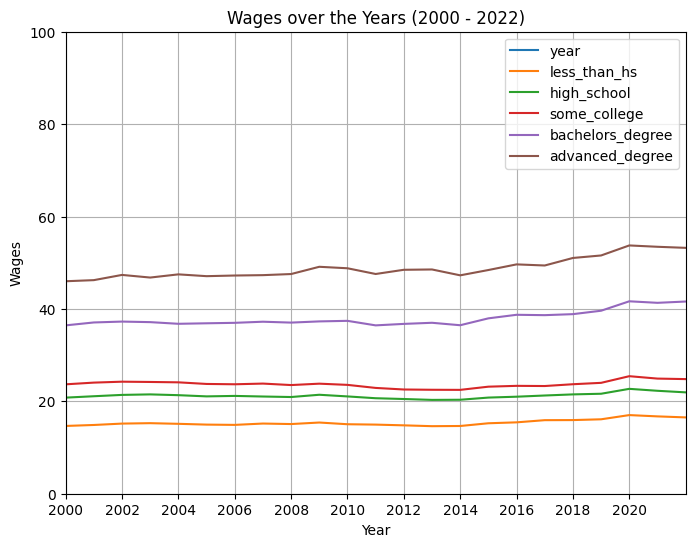
\includegraphics{Markdown_files/figure-pdf/cell-4-output-1.png}

}

\end{figure}

\begin{Shaded}
\begin{Highlighting}[]
\CommentTok{\# Making Table}
\NormalTok{statistics\_per\_column }\OperatorTok{=}\NormalTok{ \{\}}
\ControlFlowTok{for}\NormalTok{ column }\KeywordTok{in}\NormalTok{ wages\_noYear.columns:}
\NormalTok{    min\_value }\OperatorTok{=}\NormalTok{ wages\_noYear[column].}\BuiltInTok{min}\NormalTok{()}
\NormalTok{    max\_value }\OperatorTok{=}\NormalTok{ wages\_noYear[column].}\BuiltInTok{max}\NormalTok{()}
\NormalTok{    yearly\_change }\OperatorTok{=}\NormalTok{ wages\_noYear[column].diff().mean()}
\NormalTok{    wage\_total\_percent\_increase }\OperatorTok{=}\NormalTok{ ((max\_value }\OperatorTok{{-}}\NormalTok{ min\_value) }\OperatorTok{/}\NormalTok{ min\_value) }\OperatorTok{*} \DecValTok{100} \ControlFlowTok{if}\NormalTok{ min\_value }\OperatorTok{!=} \DecValTok{0} \ControlFlowTok{else} \DecValTok{0}
\NormalTok{    yearly\_change\_percent }\OperatorTok{=}\NormalTok{ ((yearly\_change}\OperatorTok{/}\NormalTok{min\_value) }\OperatorTok{*} \DecValTok{100}\NormalTok{)}

\NormalTok{    statistics\_per\_column[column] }\OperatorTok{=}\NormalTok{ \{}
        \StringTok{\textquotesingle{}Min\textquotesingle{}}\NormalTok{: }\BuiltInTok{round}\NormalTok{(min\_value, }\DecValTok{2}\NormalTok{),}
        \StringTok{\textquotesingle{}Max\textquotesingle{}}\NormalTok{: }\BuiltInTok{round}\NormalTok{(max\_value, }\DecValTok{2}\NormalTok{),}
        \StringTok{\textquotesingle{}Average Change Over Year\textquotesingle{}}\NormalTok{: }\BuiltInTok{round}\NormalTok{(yearly\_change, }\DecValTok{2}\NormalTok{),}
        \StringTok{\textquotesingle{}Average Percent Change Over Year\textquotesingle{}}\NormalTok{:}\SpecialStringTok{f"}\SpecialCharTok{\{}\BuiltInTok{round}\NormalTok{(yearly\_change\_percent, }\DecValTok{2}\NormalTok{)}\SpecialCharTok{\}}\SpecialStringTok{\%"}\NormalTok{,}
        \StringTok{\textquotesingle{}Total Percent Increase\textquotesingle{}}\NormalTok{: }\SpecialStringTok{f"}\SpecialCharTok{\{}\BuiltInTok{round}\NormalTok{(wage\_total\_percent\_increase, }\DecValTok{2}\NormalTok{)}\SpecialCharTok{\}}\SpecialStringTok{\%"}
\NormalTok{    \}}

\NormalTok{statistics\_df }\OperatorTok{=}\NormalTok{ pd.DataFrame.from\_dict(statistics\_per\_column, orient}\OperatorTok{=}\StringTok{\textquotesingle{}columns\textquotesingle{}}\NormalTok{)}
\BuiltInTok{print}\NormalTok{(statistics\_df)}
\end{Highlighting}
\end{Shaded}

\begin{verbatim}
                                 less_than_hs high_school some_college  \
Min                                     14.62       20.31        22.48   
Max                                     17.02        22.7        25.44   
Average Change Over Year                 0.08        0.05         0.05   
Average Percent Change Over Year        0.58%       0.26%        0.23%   
Total Percent Increase                 16.42%      11.77%       13.17%   

                                 bachelors_degree advanced_degree  
Min                                         36.44           45.99  
Max                                         41.65           53.74  
Average Change Over Year                     0.23            0.33  
Average Percent Change Over Year            0.64%           0.71%  
Total Percent Increase                      14.3%          16.85%  
\end{verbatim}

It is immediately visible that the wage increases are stagnant, and that
the differences between individuals with less than a high school
diploma, individuals with a high school diploma, and those who have
completed a college diploma are minor. Whereas, those who completed a
bachelor see a significant pay increase, which stands equally as true
for those who have some advanced degree. Even so, the total percent
increase per category is close to consistent across the board. One
noticeable difference is that there is less of a difference between
those with no High School diploma and those with just a High School
diploma.

The second basic metric was to graph the changes in CPI per year.
Graphing this data allows us to better visualize the changes that a
person working and living through those years would experience. The
day-to-day, or even, year-to-year changes are small; however, when
mapping on a large scale a pattern of small changes becomes a
significant outline.

\begin{Shaded}
\begin{Highlighting}[]
\CommentTok{\# Plotting line graph 2 }
\NormalTok{CPI[}\StringTok{\textquotesingle{}date\textquotesingle{}}\NormalTok{] }\OperatorTok{=}\NormalTok{ pd.to\_datetime(CPI[}\StringTok{\textquotesingle{}date\textquotesingle{}}\NormalTok{])}

\NormalTok{plt.figure(figsize}\OperatorTok{=}\NormalTok{(}\DecValTok{10}\NormalTok{, }\DecValTok{6}\NormalTok{))}
\NormalTok{plt.plot(CPI[}\StringTok{\textquotesingle{}date\textquotesingle{}}\NormalTok{], CPI[}\StringTok{\textquotesingle{}value\textquotesingle{}}\NormalTok{], marker}\OperatorTok{=}\StringTok{\textquotesingle{}o\textquotesingle{}}\NormalTok{, linestyle}\OperatorTok{=}\StringTok{\textquotesingle{}{-}\textquotesingle{}}\NormalTok{)}

\NormalTok{plt.xlabel(}\StringTok{\textquotesingle{}Date\textquotesingle{}}\NormalTok{)}
\NormalTok{plt.ylabel(}\StringTok{\textquotesingle{}CPI Value\textquotesingle{}}\NormalTok{)}
\NormalTok{plt.title(}\StringTok{\textquotesingle{}Changes in CPI over Time (January 2000 {-} December 2022)\textquotesingle{}}\NormalTok{)}
\NormalTok{plt.grid(}\VariableTok{True}\NormalTok{)}
\NormalTok{plt.xticks(rotation}\OperatorTok{=}\DecValTok{45}\NormalTok{)  }\CommentTok{\# Rotate x axis}
\NormalTok{plt.grid(}\VariableTok{True}\NormalTok{)}
\NormalTok{plt.xlim(pd.Timestamp(}\StringTok{\textquotesingle{}2000{-}01{-}01\textquotesingle{}}\NormalTok{), pd.Timestamp(}\StringTok{\textquotesingle{}2022{-}12{-}31\textquotesingle{}}\NormalTok{))}
\NormalTok{plt.ylim(}\DecValTok{0}\NormalTok{, }\DecValTok{400}\NormalTok{)}
\NormalTok{plt.show()}
\end{Highlighting}
\end{Shaded}

\begin{figure}[H]

{\centering 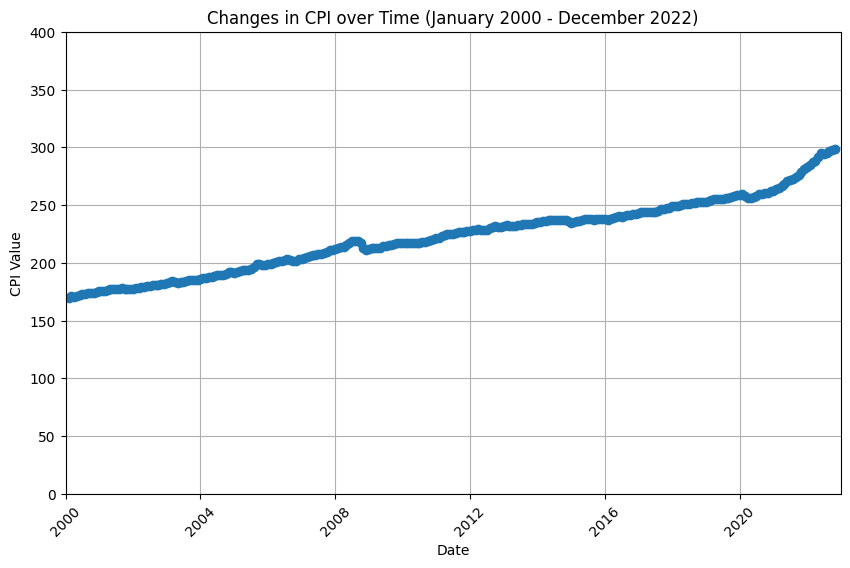
\includegraphics{Markdown_files/figure-pdf/cell-6-output-1.png}

}

\end{figure}

\begin{Shaded}
\begin{Highlighting}[]
\CommentTok{\# Calculate statistics}
\NormalTok{CPI[}\StringTok{\textquotesingle{}yearly\_change\textquotesingle{}}\NormalTok{] }\OperatorTok{=}\NormalTok{ CPI[}\StringTok{\textquotesingle{}value\textquotesingle{}}\NormalTok{].diff() }
\NormalTok{average\_change }\OperatorTok{=}\NormalTok{ CPI[}\StringTok{\textquotesingle{}yearly\_change\textquotesingle{}}\NormalTok{].mean() }
\NormalTok{average\_change }\OperatorTok{=}\NormalTok{ average\_change }\OperatorTok{*} \DecValTok{12}
\NormalTok{min\_value }\OperatorTok{=}\NormalTok{ CPI[}\StringTok{\textquotesingle{}value\textquotesingle{}}\NormalTok{].}\BuiltInTok{min}\NormalTok{()}
\NormalTok{max\_value }\OperatorTok{=}\NormalTok{ CPI[}\StringTok{\textquotesingle{}value\textquotesingle{}}\NormalTok{].}\BuiltInTok{max}\NormalTok{()}
\NormalTok{total\_change\_percent }\OperatorTok{=}\NormalTok{ ((max\_value }\OperatorTok{{-}}\NormalTok{ min\_value) }\OperatorTok{/}\NormalTok{ min\_value) }\OperatorTok{*} \DecValTok{100}
\NormalTok{CPI\_yearly\_change\_percent }\OperatorTok{=}\NormalTok{ ((average\_change}\OperatorTok{/}\NormalTok{min\_value) }\OperatorTok{*} \DecValTok{100}\NormalTok{)}


\NormalTok{statistics\_table2 }\OperatorTok{=}\NormalTok{ \{}
    \StringTok{\textquotesingle{}Min\textquotesingle{}}\NormalTok{: }\BuiltInTok{round}\NormalTok{(CPI[}\StringTok{\textquotesingle{}value\textquotesingle{}}\NormalTok{].}\BuiltInTok{min}\NormalTok{(), }\DecValTok{2}\NormalTok{),}
    \StringTok{\textquotesingle{}Max\textquotesingle{}}\NormalTok{: }\BuiltInTok{round}\NormalTok{(CPI[}\StringTok{\textquotesingle{}value\textquotesingle{}}\NormalTok{].}\BuiltInTok{max}\NormalTok{(), }\DecValTok{2}\NormalTok{),}
    \StringTok{\textquotesingle{}Average Change Over Year\textquotesingle{}}\NormalTok{: }\BuiltInTok{round}\NormalTok{(average\_change, }\DecValTok{2}\NormalTok{),}
    \StringTok{\textquotesingle{}Average Percent Change Over Year\textquotesingle{}}\NormalTok{:}\SpecialStringTok{f"}\SpecialCharTok{\{}\BuiltInTok{round}\NormalTok{(CPI\_yearly\_change\_percent, }\DecValTok{2}\NormalTok{)}\SpecialCharTok{\}}\SpecialStringTok{\%"}\NormalTok{,}
    \StringTok{"Total Percent Increase"}\NormalTok{ : }\SpecialStringTok{f"}\SpecialCharTok{\{}\BuiltInTok{round}\NormalTok{(total\_change\_percent)}\SpecialCharTok{\}}\SpecialStringTok{\%"}

\NormalTok{\}}

\CommentTok{\# Table}
\NormalTok{table2 }\OperatorTok{=}\NormalTok{ pd.DataFrame.from\_dict(statistics\_table2, orient}\OperatorTok{=}\StringTok{\textquotesingle{}index\textquotesingle{}}\NormalTok{, columns}\OperatorTok{=}\NormalTok{[}\StringTok{\textquotesingle{}Values\textquotesingle{}}\NormalTok{])}
\BuiltInTok{print}\NormalTok{(table2)}
\end{Highlighting}
\end{Shaded}

\begin{verbatim}
                                 Values
Min                               170.0
Max                               298.6
Average Change Over Year           5.65
Average Percent Change Over Year  3.33%
Total Percent Increase              76%
\end{verbatim}

After creating the data frames and table, it is easily visible that the
Consumer Price Index changes at an average of 3.33\% a year, for a total
of 76\%. A staggering increase compared to the average wage increase
year over year. The inability of wages to keep up with inflation can
lead to a decrease in the standard of living for affected individuals or
households. They may have to allocate more of their income towards
essentials like housing, food, and healthcare, leaving less for savings
or discretionary spending.

This scenario can lead to financial stress, especially for those on
fixed incomes or with limited opportunities for wage increases. It might
force individuals to cut back on non-essential expenses or seek
additional sources of income to maintain their previous standard of
living. A frightening outlook on the future. What is obvious when
looking at both of these data visualizations is that they have little
variation year over year, leading me to predict that this pattern will
likely remain constant.

On the question of whether or not there has been a consistent
relationship between the CPI and wage growth over the past two decades,
I decided to plot the percentage increase yearly for all of the tracked
metrics in this paper. The following graph represents the data visible
in the tables. It enables the visualization of how daunting the
differences have been.

\begin{Shaded}
\begin{Highlighting}[]
\CommentTok{\# Merging data}
\NormalTok{CPI[}\StringTok{\textquotesingle{}date\textquotesingle{}}\NormalTok{] }\OperatorTok{=}\NormalTok{ pd.to\_datetime(CPI[}\StringTok{\textquotesingle{}date\textquotesingle{}}\NormalTok{])}
\NormalTok{CPI\_yearly }\OperatorTok{=}\NormalTok{ CPI.groupby(CPI[}\StringTok{\textquotesingle{}date\textquotesingle{}}\NormalTok{].dt.year).first()}
\NormalTok{CPI\_yearly.index.name }\OperatorTok{=} \StringTok{\textquotesingle{}year\textquotesingle{}}
\NormalTok{CPI\_yearly.reset\_index(inplace}\OperatorTok{=}\VariableTok{True}\NormalTok{)}

\NormalTok{CPI\_values }\OperatorTok{=}\NormalTok{ CPI\_yearly[}\StringTok{\textquotesingle{}value\textquotesingle{}}\NormalTok{]}
\NormalTok{wages\_with\_CPI }\OperatorTok{=}\NormalTok{ wages.join(CPI\_values, how}\OperatorTok{=}\StringTok{\textquotesingle{}inner\textquotesingle{}}\NormalTok{)}
\NormalTok{wages\_with\_CPI[}\StringTok{\textquotesingle{}value\textquotesingle{}}\NormalTok{] }\OperatorTok{=}\NormalTok{ wages\_with\_CPI[}\StringTok{\textquotesingle{}value\textquotesingle{}}\NormalTok{].iloc[::}\OperatorTok{{-}}\DecValTok{1}\NormalTok{]}

\CommentTok{\# Calculate the percentage diff}
\NormalTok{wages\_with\_CPI[}\StringTok{\textquotesingle{}value\textquotesingle{}}\NormalTok{] }\OperatorTok{=}\NormalTok{ wages\_with\_CPI[}\StringTok{\textquotesingle{}value\textquotesingle{}}\NormalTok{].values[::}\OperatorTok{{-}}\DecValTok{1}\NormalTok{]}
\NormalTok{wages\_with\_CPI }\OperatorTok{=}\NormalTok{ wages\_with\_CPI.rename(columns}\OperatorTok{=}\NormalTok{\{}\StringTok{\textquotesingle{}value\textquotesingle{}}\NormalTok{: }\StringTok{\textquotesingle{}CPI\textquotesingle{}}\NormalTok{\})}

\CommentTok{\# Calculate the percentage diff}
\NormalTok{percentage\_diff }\OperatorTok{=}\NormalTok{ wages\_with\_CPI.drop(}\StringTok{\textquotesingle{}year\textquotesingle{}}\NormalTok{, axis}\OperatorTok{=}\DecValTok{1}\NormalTok{).}\BuiltInTok{apply}\NormalTok{(}\KeywordTok{lambda}\NormalTok{ x: ((x }\OperatorTok{{-}}\NormalTok{ x.}\BuiltInTok{min}\NormalTok{()) }\OperatorTok{/}\NormalTok{ x.}\BuiltInTok{min}\NormalTok{()) }\OperatorTok{*} \DecValTok{100}\NormalTok{)}

\NormalTok{plt.figure(figsize}\OperatorTok{=}\NormalTok{(}\DecValTok{8}\NormalTok{, }\DecValTok{6}\NormalTok{))}

\CommentTok{\# Plotting the percentage difference for each column}
\ControlFlowTok{for}\NormalTok{ column }\KeywordTok{in}\NormalTok{ percentage\_diff.columns:}
    \ControlFlowTok{if}\NormalTok{ column }\OperatorTok{!=} \StringTok{\textquotesingle{}year\textquotesingle{}}\NormalTok{:  }
\NormalTok{        plt.plot(wages\_with\_CPI[}\StringTok{\textquotesingle{}year\textquotesingle{}}\NormalTok{], percentage\_diff[column], label}\OperatorTok{=}\NormalTok{column)}

\NormalTok{plt.xlabel(}\StringTok{\textquotesingle{}Year\textquotesingle{}}\NormalTok{)}
\NormalTok{plt.ylabel(}\StringTok{\textquotesingle{}\% Difference from Minimum\textquotesingle{}}\NormalTok{)}
\NormalTok{plt.title(}\StringTok{\textquotesingle{}Percentage Difference from Minimum Value by Year\textquotesingle{}}\NormalTok{)}
\NormalTok{plt.ylim(}\DecValTok{0}\NormalTok{, }\DecValTok{100}\NormalTok{)}
\NormalTok{plt.xlim(}\DecValTok{2000}\NormalTok{, }\DecValTok{2022}\NormalTok{)}
\NormalTok{plt.legend()}
\NormalTok{plt.grid(}\VariableTok{True}\NormalTok{)}
\NormalTok{plt.show()}
\end{Highlighting}
\end{Shaded}

\begin{figure}[H]

{\centering 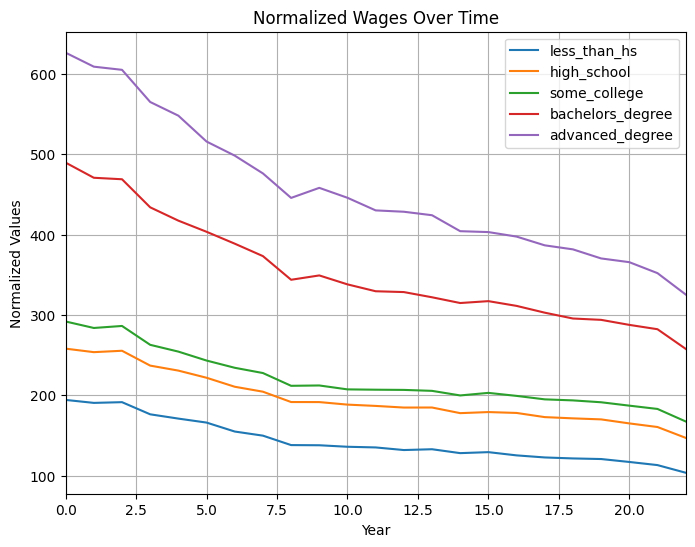
\includegraphics{Markdown_files/figure-pdf/cell-8-output-1.png}

}

\end{figure}

Next, I inquired about the difference in purchasing power in 2000 to
2022 based on education levels. My method was dividing income by CPI. To
do so I first multiplied every income by 2000 hours, an estimation of
full-time pay based on the following assumptions: Weekly Hours × Weeks
Worked per Year=Annual Hours Worked. 40 hours/week × 50 weeks/year =
2000 hours/year.

\begin{Shaded}
\begin{Highlighting}[]
\NormalTok{columns\_to\_multiply }\OperatorTok{=}\NormalTok{ [}\StringTok{\textquotesingle{}less\_than\_hs\textquotesingle{}}\NormalTok{, }\StringTok{\textquotesingle{}high\_school\textquotesingle{}}\NormalTok{, }\StringTok{\textquotesingle{}some\_college\textquotesingle{}}\NormalTok{, }\StringTok{\textquotesingle{}bachelors\_degree\textquotesingle{}}\NormalTok{, }\StringTok{\textquotesingle{}advanced\_degree\textquotesingle{}}\NormalTok{]}

\CommentTok{\# Multiplying selected columns by 2000}
\NormalTok{wages\_with\_CPI[columns\_to\_multiply] }\OperatorTok{*=} \DecValTok{2000}

\NormalTok{wagesYear }\OperatorTok{=}\NormalTok{ wages\_with\_CPI.join(CPI\_values, how}\OperatorTok{=}\StringTok{\textquotesingle{}inner\textquotesingle{}}\NormalTok{)}

\CommentTok{\# Dividing wage columns by \textquotesingle{}CPI\textquotesingle{}}
\NormalTok{wagesYear\_normalized }\OperatorTok{=}\NormalTok{ wagesYear[columns\_to\_multiply].div(wagesYear[}\StringTok{\textquotesingle{}value\textquotesingle{}}\NormalTok{], axis}\OperatorTok{=}\DecValTok{0}\NormalTok{)}

\NormalTok{plt.figure(figsize}\OperatorTok{=}\NormalTok{(}\DecValTok{8}\NormalTok{, }\DecValTok{6}\NormalTok{))}

\ControlFlowTok{for}\NormalTok{ column }\KeywordTok{in}\NormalTok{ wagesYear\_normalized.columns:}
\NormalTok{    plt.plot(wagesYear.index, wagesYear\_normalized[column], label}\OperatorTok{=}\NormalTok{column)}

\NormalTok{plt.xlabel(}\StringTok{\textquotesingle{}Year\textquotesingle{}}\NormalTok{)}
\NormalTok{plt.ylabel(}\StringTok{\textquotesingle{}Normalized Values\textquotesingle{}}\NormalTok{)}
\NormalTok{plt.title(}\StringTok{\textquotesingle{}Normalized Wages Over Time\textquotesingle{}}\NormalTok{)}
\NormalTok{plt.xlim(}\DecValTok{0}\NormalTok{, }\DecValTok{22}\NormalTok{)}
\NormalTok{plt.legend()}
\NormalTok{plt.grid(}\VariableTok{True}\NormalTok{)}
\NormalTok{plt.show()}
\end{Highlighting}
\end{Shaded}

\begin{figure}[H]

{\centering 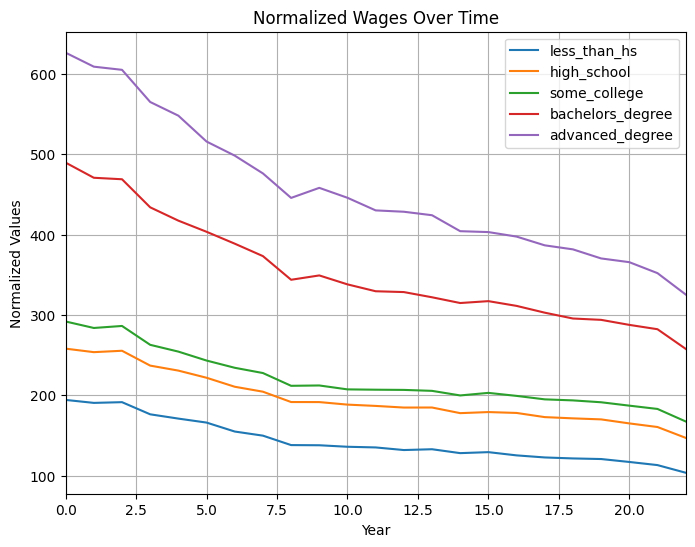
\includegraphics{Markdown_files/figure-pdf/cell-9-output-1.png}

}

\end{figure}

\begin{Shaded}
\begin{Highlighting}[]
\CommentTok{\# Last table}
\NormalTok{statistics\_per\_column }\OperatorTok{=}\NormalTok{ \{\}}
\ControlFlowTok{for}\NormalTok{ column }\KeywordTok{in}\NormalTok{ wagesYear\_normalized.columns:}
\NormalTok{    min\_value }\OperatorTok{=}\NormalTok{ wagesYear\_normalized[column].}\BuiltInTok{min}\NormalTok{()}
\NormalTok{    max\_value }\OperatorTok{=}\NormalTok{ wagesYear\_normalized[column].}\BuiltInTok{max}\NormalTok{()}
\NormalTok{    yearly\_change }\OperatorTok{=}\NormalTok{ wagesYear\_normalized[column].diff().mean()}
\NormalTok{    wage\_total\_percent\_increase }\OperatorTok{=}\NormalTok{ ((max\_value }\OperatorTok{{-}}\NormalTok{ min\_value) }\OperatorTok{/}\NormalTok{ min\_value) }\OperatorTok{*} \DecValTok{100} \ControlFlowTok{if}\NormalTok{ min\_value }\OperatorTok{!=} \DecValTok{0} \ControlFlowTok{else} \DecValTok{0}
\NormalTok{    yearly\_change\_percent }\OperatorTok{=}\NormalTok{ ((yearly\_change}\OperatorTok{/}\NormalTok{min\_value) }\OperatorTok{*} \DecValTok{100}\NormalTok{)}

\NormalTok{    statistics\_per\_column[column] }\OperatorTok{=}\NormalTok{ \{}
        \StringTok{\textquotesingle{}Min\textquotesingle{}}\NormalTok{: }\BuiltInTok{round}\NormalTok{(min\_value, }\DecValTok{2}\NormalTok{),}
        \StringTok{\textquotesingle{}Max\textquotesingle{}}\NormalTok{: }\BuiltInTok{round}\NormalTok{(max\_value, }\DecValTok{2}\NormalTok{),}
        \StringTok{\textquotesingle{}Average Change Over Year\textquotesingle{}}\NormalTok{: }\BuiltInTok{round}\NormalTok{(yearly\_change, }\DecValTok{2}\NormalTok{),}
        \StringTok{\textquotesingle{}Average Percent Change Over Year\textquotesingle{}}\NormalTok{:}\SpecialStringTok{f"}\SpecialCharTok{\{}\BuiltInTok{round}\NormalTok{(yearly\_change\_percent, }\DecValTok{2}\NormalTok{)}\SpecialCharTok{\}}\SpecialStringTok{\%"}\NormalTok{,}
        \StringTok{\textquotesingle{}Total Percent Change\textquotesingle{}}\NormalTok{: }\SpecialStringTok{f"}\SpecialCharTok{\{}\BuiltInTok{round}\NormalTok{(wage\_total\_percent\_increase, }\DecValTok{2}\NormalTok{)}\SpecialCharTok{\}}\SpecialStringTok{\%"}
\NormalTok{    \}}

\NormalTok{statistics\_df }\OperatorTok{=}\NormalTok{ pd.DataFrame.from\_dict(statistics\_per\_column, orient}\OperatorTok{=}\StringTok{\textquotesingle{}columns\textquotesingle{}}\NormalTok{)}
\BuiltInTok{print}\NormalTok{(statistics\_df)}
\end{Highlighting}
\end{Shaded}

\begin{verbatim}
                                 less_than_hs high_school some_college  \
Min                                    103.82      147.21       167.59   
Max                                    194.35      258.12       291.88   
Average Change Over Year                 4.12        5.04         5.65   
Average Percent Change Over Year        3.96%       3.42%        3.37%   
Total Percent Change                    87.2%      75.35%       74.17%   

                                 bachelors_degree advanced_degree  
Min                                        257.89          325.48  
Max                                        489.41          626.12  
Average Change Over Year                    10.52           13.67  
Average Percent Change Over Year            4.08%            4.2%  
Total Percent Change                       89.77%          92.37%  
\end{verbatim}

As we can see from the table, the average divergence at the end of the
twenty-two-year period was 83.77\%. This means an average individual's
purchasing power would translate to every 100 dollars earned today being
worth 183.77 dollars in the year 2000.

To answer my question ``Which levels of education have shown the
strongest correlation between wage changes and CPI variations since
2000?'' it seems to be that having a college none-bachelors degree is
the smallest difference in purchasing power. With that said, no
education level had any meaningful correlation to CPI.

The trends analyzed today are consistent. Wages have on average
increased by around 4 dollars an hour, while the Consumer Price Index
has changed by 128 points approximately.

\hypertarget{final-thoughts}{%
\subsection{Final Thoughts}\label{final-thoughts}}

Throughout this analysis, we delved into the intricate dynamics between
CPI variations and wage fluctuations across different educational strata
from 2000 to 2022. Utilizing statistical analysis, primarily employing
Python's Pandas library, we uncovered compelling insights into the
impact of inflation on purchasing power and income disparities.

Our findings highlighted a discernible disparity in the adjustment of
wages across educational levels in response to CPI changes. It became
evident that while certain sectors or educational groups showcased minor
resilience to CPI fluctuations, they all experienced disproportionate
impacts on real wages.

The data underscored the crucial role education plays in buffering
individuals by providing higher wages; despite not being indicative of
correlation to CPI. However, disparities persisted, revealing the need
for targeted interventions to mitigate income inequalities stemming from
CPI variations.

Our analysis elucidated the nuanced interplay between CPI, wage
adjustments, and their implications for economic policies and societal
well-being. The inability of wages to consistently keep pace with CPI
growth underscored the challenges individuals face in maintaining
purchasing power and sustaining their standard of living.

Moving forward, these findings prompt a reconsideration of policy
frameworks aimed at addressing wage stagnation, bolstering educational
opportunities, and ensuring a more equitable distribution of income.
Furthermore, this analysis puts into evidence the need for further
research into the multifaceted relationship between inflation,
education, and income dynamics, paving the way for more informed
economic strategies and social policies.

\hypertarget{works-cited}{%
\subsection{Works Cited}\label{works-cited}}

Asaniczka. ``Wages by Education in the USA (1973-2022).'' Kaggle, 5
Dec.~2023,
www.kaggle.com/datasets/asaniczka/wages-by-education-in-the-usa-1973-2022.

Narne, Pavan. ``US Inflation Dataset (1947 - 2023).'' Kaggle, 30 July
2023,
www.kaggle.com/datasets/pavankrishnanarne/us-inflation-dataset-1947-present.



\end{document}
